\tikzstyle{pvalue}=[circle, draw, fill=blue!50, minimum height=3em]
\tikzstyle{ovalue}=[circle, draw,fill=red!50, minimum height=3em]
\tikzstyle{dcell}=[circle,draw, minimum height=1em]
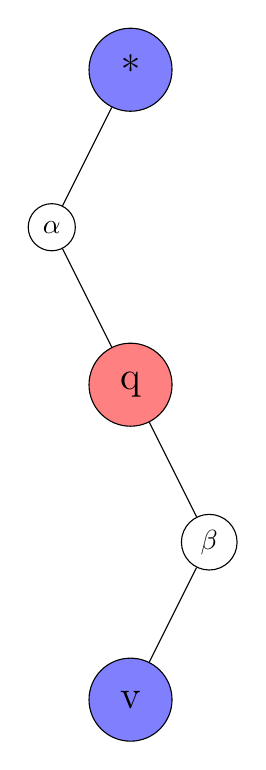
\begin{tikzpicture}

\node [pvalue] (v1) at (-2,0) {\Large{*}};
\node [dcell] (v2) at (-3,-2) {$\alpha$};
\node [ovalue] (v3) at (-2,-4) {\Large{q}};
\node [dcell] (v4) at (-1,-6) {$\beta$};
\node [pvalue] (v5) at (-2,-8) {\Large{v}};
\draw  (v1) edge (v2);
\draw  (v2) edge (v3);
\draw  (v3) edge (v4);
\draw  (v4) edge (v5);
\end{tikzpicture}